\documentclass[11pt,reqno]{amsart}
%\pagestyle{empty} 
\setlength{\topmargin}{-0.5in} % usually -0.25in
\addtolength{\textheight}{1.2in} % usually 1.25in
\addtolength{\oddsidemargin}{-0.8in}
\addtolength{\evensidemargin}{-0.8in}
\addtolength{\textwidth}{1.6in} %\setlength{\parindent}{0pt}

\newcommand{\normalspacing}{\renewcommand{\baselinestretch}{1.1}\tiny\normalsize}
\normalspacing

% macros
\usepackage{amssymb,xspace,alltt,verbatim}
\usepackage[final]{graphicx}
\usepackage[pdftex,colorlinks=true]{hyperref}
\usepackage{fancyvrb}

\usepackage{fancyhdr}
\pagestyle{fancy}

\usepackage{tikz}
\usetikzlibrary{shapes}

\newtheorem*{lem*}{Lemma}

\newcommand{\ba}{\mathbf{a}}
\newcommand{\bb}{\mathbf{b}}
\newcommand{\bc}{\mathbf{c}}
\newcommand{\bbf}{\mathbf{f}}
\newcommand{\bi}{\mathbf{i}}
\newcommand{\bj}{\mathbf{j}}
\newcommand{\bk}{\mathbf{k}}
\newcommand{\bn}{\mathbf{n}}
\newcommand{\br}{\mathbf{r}}
\newcommand{\bs}{\mathbf{s}}
\newcommand{\bu}{\mathbf{u}}
\newcommand{\bv}{\mathbf{v}}
\newcommand{\bx}{\mathbf{x}}

\newcommand{\bF}{\mathbf{F}}

\newcommand{\CC}{{\mathbb{C}}}
\newcommand{\RR}{{\mathbb{R}}}
\newcommand{\eps}{\epsilon}
\newcommand{\ZZ}{{\mathbb{Z}}}
\newcommand{\NN}{{\mathbb{N}}}
\newcommand{\ip}[2]{\mathrm{\left<#1,#2\right>}}
\newcommand{\grad}{\nabla}

\newcommand{\dydx}{\frac{dy}{dx}}

\newcommand{\Matlab}{\textsc{Matlab}\xspace}
\newcommand{\Octave}{\textsc{Octave}\xspace}

\newcommand{\prob}[1]{\bigskip\noindent\textbf{#1.} }
\newcommand{\pts}[1]{(\emph{#1 pts})}

\newcommand{\probpts}[2]{\prob{#1} \pts{#2} \,\,}
\newcommand{\ppartpts}[2]{\textbf{(#1)} \pts{#2} \,\,}
\newcommand{\epartpts}[2]{\medskip\noindent \textbf{(#1)} \pts{#2} \,\,}

\newcommand*\circled[1]{\tikz[baseline=(char.base)]{
            \node[shape=ellipse,draw,inner sep=2pt] (char) {#1};}}

\lhead{MATH F302 UX1: \textsl{SAMPLE} Midterm 1}

\rhead{\thepage}

\cfoot{}

\begin{document}
\hfill \Large Name:\underline{\phantom{Ed Bueler really really long long long name}}
\medskip

\scriptsize \noindent MATH F302 UX1 Differential Equations (Bueler) \hfill 19--21 February 2019
\medskip

\Large\centerline{\textbf{\textsl{SAMPLE} Midterm 1}}

\medskip
\large
\begin{center}
\textbf{Proctored.  90 minutes.  100 points total.  No textbook or notes or calculator.  When it makes sense to do so, please \circled{circle} your final answer(s).}
\end{center}

\bigskip
\thispagestyle{empty}
\normalsize

\probpts{1}{2}  Show that $6 y^{1/3} - x^2 = 7$ defines an implicit solution to the ODE
	$$\dydx = x y^{2/3}$$
\vfill

\probpts{Extra Credit}{5}  Note $6 y^{1/3} - x^2 = 0$ also defines a solution to the DE in the above problem.  Show this solution passes through $(0,0)$.  Then find another solution to the same DE which also passes through $(0,0)$.  Explain why this situation is \emph{not} a violation of the theorem on existence and uniqueness for initial value problems.
\vfill

\prob{1} \ppartpts{a}{2}  The ODE 
	$$\dydx = xy$$
has the direction field shown below.  Sketch the solution to this ODE which passes through $(x_0,y_0)=(0,2)$.

\bigskip
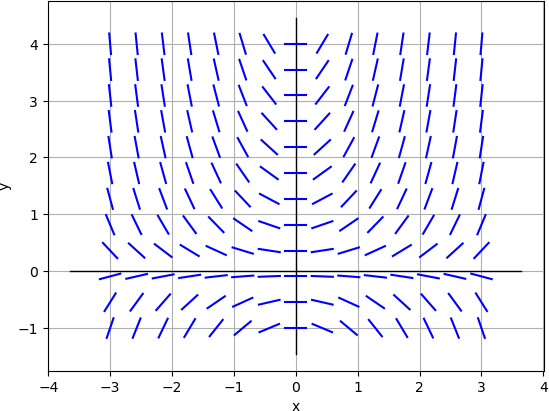
\includegraphics[width=0.4\textwidth]{dirfieldxy}
\vfill

\epartpts{b}{5}  Solve the following initial value problem---\emph{give an exact formula $y(x)$ for the solution!}---and then sketch the solution you find on the direction field above:
	$$\dydx = xy, \qquad y(1)=1.$$
\vfill

% ?
\prob{1} \ppartpts{a}{2}  Show that the following equation is exact:
	$$\frac{t}{y}\,dy + (1+\ln y)\,dt = 0.$$
\vfill

\epartpts{b}{5}  Solve the ordinary differential equation in part \textbf{(a)}.  Write the solution as an explicit formula for $y(t)$.
\vfill


\probpts{2}{7}  Find the solution to the initial value problem:
	$$\dydx + 2y = e^{-x}, \qquad y(-1)=e.$$
\vfill


\newpage
\probpts{3}{7}  Use Euler's method to approximate the solution to the initial value problem at the points $x=0.1$ and $x=0.2$, with steps of size $h=0.1$:
	$$\dydx = x+ y, \qquad y(0)=1.$$
\vfill

\probpts{3}{7}  Find the general solution
	$$\frac{dz}{dt} = \frac{t-5}{z^2-z}$$
\vfill

\prob{7}  Recall that Newton's law of cooling is the DE
\begin{equation}
    \frac{dT}{dt} = k (T_m - T) \label{newton}
\end{equation}
where $T(t)$ is the temperature of the object, $T_m$ is the ambient temperature, and $k$ is a positive constant.

\ppartpts{a}{2}  Suppose that at $t=0$ a glass of water at room temperature, say $70\,{}^\circ$F, is taken outside when it is $40\,{}^\circ$F.  Suppose that for this glass of water, $k=0.01$, and that we measure time in minutes.  Including \eqref{newton}, write a concrete ODE IVP (i.e.~initial value problem) for this situation.
\vfill

\epartpts{b}{2}  A more realistic situation is that we do know the ambient temperature---again assume it is $40\,{}^\circ$F---but that we don't know $k$ for the glass of water.  However, we measure that the water is at temperature $58\,{}^\circ$F after $3$ minutes.  Determine $k$.  (\emph{Hint}.  You will need to solve \eqref{newton}.  You can leave your answer as a formula for a specific number; you would need a calculator to get a decimal value.)
\vfill



\noindent \hrulefill

\scriptsize \centerline{ \textsc{space available for computations \hspace{30mm} clearly label anything you want graded}}
\vspace{5.0in}
\end{document}
